\RequirePackage[l2tabu, orthodox]{nag}

\documentclass{article}

\usepackage[utf8]{inputenc}
\usepackage[ngerman]{babel}

\usepackage{natbib}
\usepackage{graphicx}
\usepackage{capt-of}
\usepackage[colorlinks,pdfpagelabels,pdfstartview=FitH,bookmarksopen=true,bookmarksnumbered=true,linkcolor=black,plainpages=false,hypertexnames=false,citecolor=black]{hyperref}
\usepackage{caption}
\usepackage{subfigure}
\usepackage{listings}
\usepackage{microtype}

% http://tex.stackexchange.com/questions/167948/package-rerunfilecheck-warning-file-out-has-changed
\usepackage{bookmark}

% gantt charts: http://ctan.mirrorcatalogs.com/graphics/pgf/contrib/pgfgantt/pgfgantt.pdf
\usepackage{pgfgantt}

% change margins to 2.5 cm
\usepackage[margin=3cm]{geometry}

% place figures at exactly the position given in the code
\usepackage{float}

\newcommand{\appname}{Flashcard-Website}


\begin{document}
\begin{titlepage}
    \large
    \begin{flushleft}
        Web Engineering, 2. Semester \\
        Projektmanagment, 2. Semester
        TINF13B2
    \end{flushleft}
    
    \vfill

    \begin{center}
    	% H. Balzert, Lehrbuch der Software-Technik
        \Huge SOLL-/IST-Analyse\\
        \Large \appname \\
        \vspace{1cm}
        \normalsize David Ehlen, \\Julien Hadley Jack, \\Sebastian Dernbach, \\
        \vspace\medskipamount
        \vspace\medskipamount
        Karlsruhe, 04.07.2014
    \end{center}
    
    \vfill
    
    \begin{flushright}
        Duale Hochschule \\
        Baden-Württemberg \\
        \vspace\medskipamount
        Betreuer: Jörn Eisenbiegler,\\
        Simone Freudenmann
    \end{flushright}
\end{titlepage}

\newpage

% removes the page numbers for the toc
\pagestyle{empty}
\addtocontents{toc}{\protect\thispagestyle{empty}}
\tableofcontents
\cleardoublepage

% normal page numbering for the rest of the document
\setcounter{page}{1}
\pagestyle{plain}
\setcounter{page}{1}

\section{Anforderungen}
\subsection{Pflichtkriterien}
\subsection{Wunschkriterien}

\section{Qualität}


\section{Projektplanung}

\section{Kosten}

\begin{figure}[H]
    \centering
    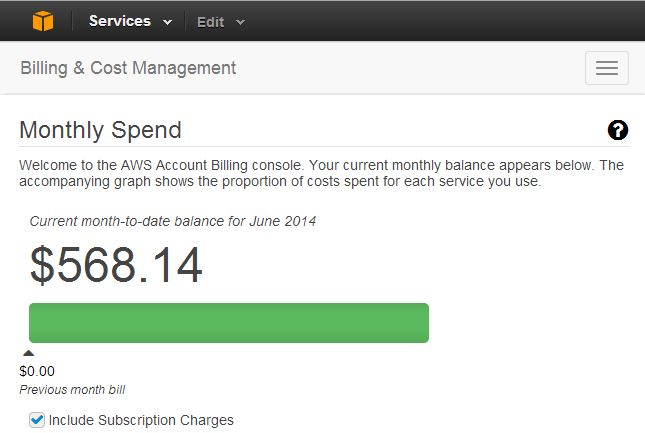
\includegraphics[width=0.7\textwidth]{images/amazon-bill.jpg}
    \caption{Hauptbildschirm}
    \label{fig:overview}
\end{figure}

\section{Risiken}

\section{Persönliche Einschätzung}

\section{Ehrenamtliche Erklärung}

Ich erkläre ehrenwörtlich,
\begin{itemize}
    \item dass ich meine Projektarbeit selbständig geplant und durchgeführt habe;
    \item dass ich die Übernahme wörtlicher Zitate aus der Literatur sowie die Verwendung der Gedanken anderer Autoren an den entsprechenden Stellen innerhalb der Arbeit gekennzeichnet habe;
    \item dass ich meine Projektarbeit bei keiner anderen Prüfung
    vorgelegt habe.
\end{itemize}
Ich bin mir bewusst, dass eine falsche Erklärung rechtliche Folgen haben wird."" \\

\vspace{1cm}
Karlsruhe, 05.07.2014 

\end{document}